\subsection{How Bonsai.ML started}

\begin{frame}
    \frametitle{AEON project}

    We are building a new type of experimentation:
    continual recording of behavioral and neural data of mice foraging in large
    arenas for weeks to months.

    \begin{center}
        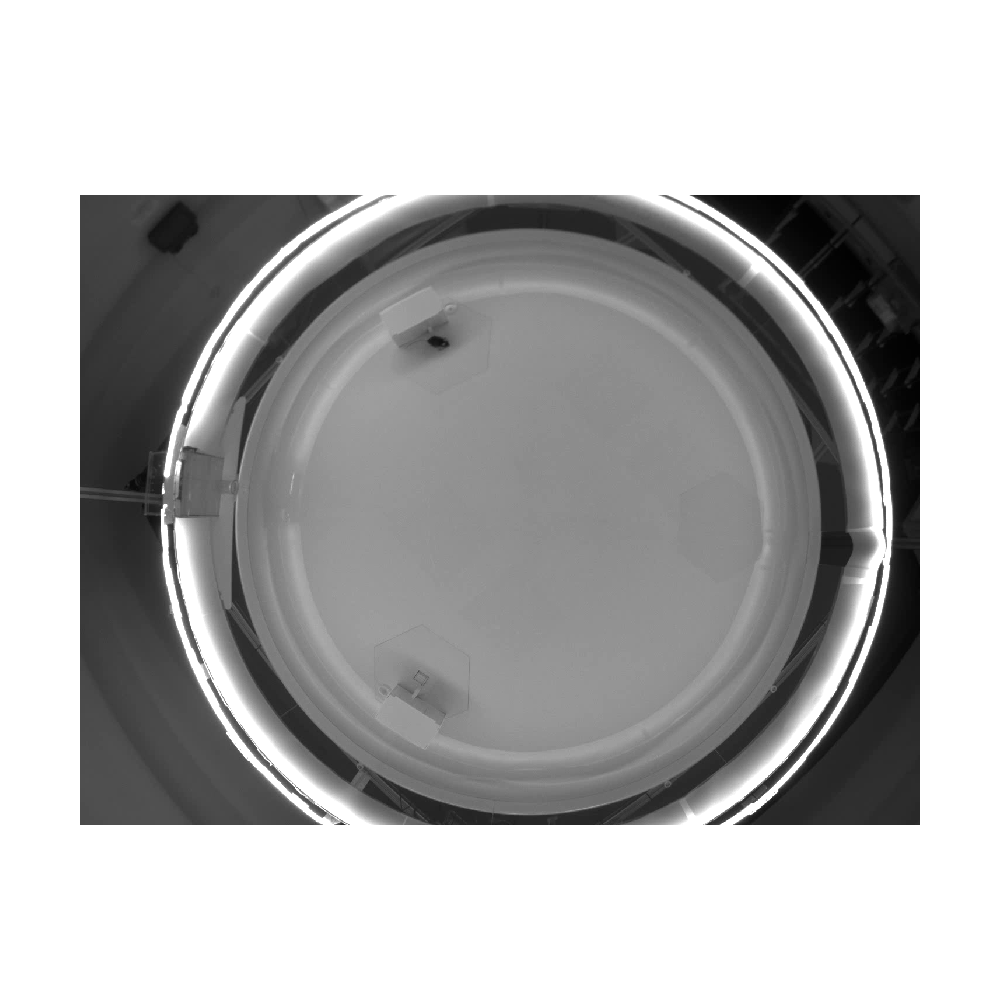
\includegraphics[width=2in]{figures/foragingMouse.png}
        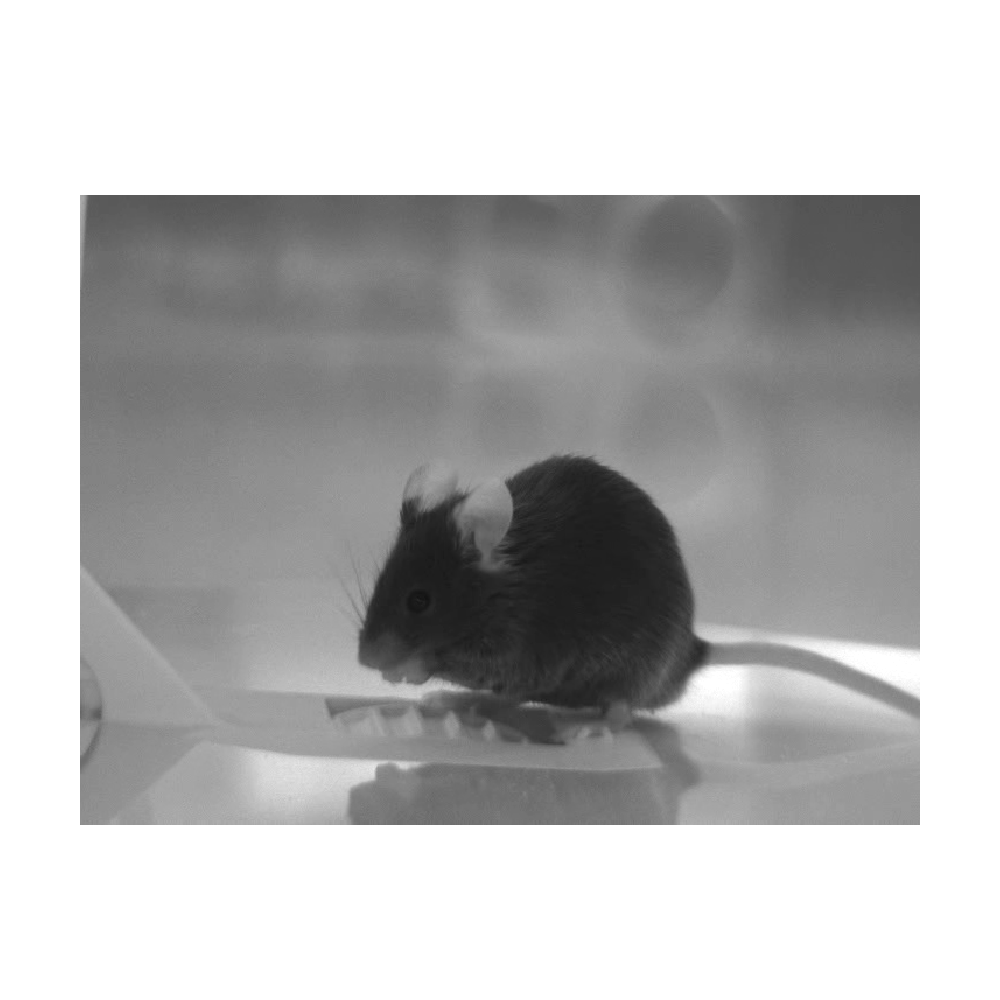
\includegraphics[width=2in]{figures/mouseOnWheel.png}
    \end{center}

\end{frame}

\begin{frame}
    \frametitle{BBSRC grant: Machine learning for Neuroscience experimental
    control}

    \textcolor{red}{Abstract}

    \tiny
    To understand the brain, scientists aim to explain how animal behaviour
    relates to neural activity. This requires the design and precise control of
    behavioural experiments, wherein animals perform particular tasks while
    experimenters either record or manipulate neural activity in specific
    neural circuits. Such experiments require data acquisition software that
    integrates and controls hardware from multiple recording devices (cameras,
    electrodes, sensors), and analysis tools that can interpret large and
    complex datasets. Progress is held back by the lack of standardised tools
    for design and implementation of experimental protocols, and the difficulty
    of integrating state-of-the-art data processing and neuroinformatics into
    custom experimental designs. The fields of behavioural and brain sciences
    have consequently suffered from both inefficiency and poor reproducibility,
    due to disparate data acquisition and analysis solutions created
    independently across laboratories. To address these challenges, we propose
    to extend, enhance, maintain and support \textbf{Bonsai}, a fully
    integrated software environment to enable cutting-edge reproducible systems
    neuroscience experiments using animal models, with a particular emphasis on
    machine-intelligence-enabled, real-time neuroinformatics methods. While
    Bonsai is already adopted by hundreds of scientists worldwide, we aim to
    extend Bonsai's functionality with a toolbox of online and offline Machine
    Intelligence tools for analysis of behavioural and neural data (video-based
    analysis of behavioural motifs, real-time and offline analysis of neural
    signals), and create an open-access platform for software sharing and
    integration with multiple programming languages. Enhancing Bonsai's
    ecosystem will be a game-changer for behavioural and brain science
    experiments by enabling new types of research, increasing and diversifying
    user base, and dramatically improve efficiency and reproducibility of
    research.

    \hfill\href{https://gow.bbsrc.ukri.org/grants/AwardDetails.aspx?FundingReference=BB\%2FW019132\%2F1}{grant
    details}

\end{frame}

\note[itemize]{
    \item at the time of the grant I did not know much about Bonsai, and I did not want to know about it because it was a Windows software
    \item but the grant reviewers helped me understand how good Bonsai was :)
    \item controlling experiments using advanced machine learning methods
        \begin{itemize}
            \item e.g., testing causality of neural patterns on behavior; deactivate a brain region when you forecast the appearance of a pattern of brain activity related to a given behavior, and check if after the deactivation the behavioral pattern disappears
            \item  e.g., only visually stimulate an animal until you achieve a certain precision in the receptive field estimation
        \end{itemize}
}

\begin{frame}
    \frametitle{My experience in machine learning and Neuroscience}

    I have developed methods for:

    \begin{itemize}

        \item nonlinear regression methods to estimate receptive fields of
            visual cells~\citep{rapelaEtAl06,rapelaEtAl10},

        \item Bayesian linear regression methods to understand the relation
            between phase concentration in the human EEG and
            attention~\citep{rapelaEtAl12-attentionSwitch,rapelaEtAl12-eyeTracking,rapelaEtAl18-avshift},

        \item dynamical systems models to model the relation between ECoG
            measurements and speech production in
            humans~\citep{rapelaInPrepTWsInSpeech,rapelaInPrepSyncTWs,rapelaInPrepSyncTWsII},

        \item unsupervised models to characterize epilepsy using Utah array
            recordings from
            humans~\citep{rapelaEtAl19-epilepsy-tsne,rapelaAndTodorov19-epilepsy-hmm}.

    \end{itemize}

    and I am the main developer of
    \href{https://github.com/joacorapela/svGPFA}{svGPFA}, a method using
    variational inference on Gaussian processes to infer latent variables from
    Neuropixels population recordings.

\end{frame}

\begin{frame}
    \frametitle{What type of machine learning we want for Bonsai?}

    \begin{description}

        \item[supervised, unsupervised and reinforcement methods]\mbox{}\\

            \begin{description}

                \item[supervised methods] find mappings between inputs X and outputs y, like in curve fitting

                \item[unsupervised methods] discover structure in inputs X, without any output, like in clustering

                \item[reinforcement learning methods] learn relations between inputs X and actions a to maximize future rewards.

            \end{description}

        \item[batch vs online processing]\mbox{}\\

            \begin{description}

                \item[batch processing] all data is read (generally from files)
                    and processed at the same time.

                \item[online processing] data is processes as it arrives and
                    processed one at a time

            \end{description}

    \end{description}

\end{frame}

\begin{frame}
    \frametitle{What type of machine learning we want for Bonsai?}

    \begin{description}

        \item[stationary vs non-stationary data]\mbox{}\\

            \begin{description}

                \item[stationary data] has statistics (i.e., characteristics)
                    that do not change with time.

                \item[non-stationary data] has time-varying statistics.

            \end{description}

        \item[iid vs time-series datasets]\mbox{}\\

            \begin{description}

                \item[iid datasets] contain samples that are unrelated (i.e., independent) from each other and all come from the same distribution. For example a dataset of coin tosses is iid.

                \item[time-series datasets] contain samples that are related to each other. For example a dataset of frames from a movie is a time-series one.

            \end{description}

    \end{description}

\end{frame}

\begin{frame}
    \frametitle{What type of machine learning we want for Bonsai?}

    \begin{description}

        \item[probabilistic vs deterministic models]\mbox{}\\

            \begin{description}

                \item[probabilistic models] assume that variables of interest are random
      quantities, and seek to estimate their distribution.

                \item[deterministic models]treat their variables of interest as deterministic
      quantitities.

            \end{description}

  \item[reactive vs non-reactive models]\mbox{}\\

            \begin{description}

            \item[non-reactive inference models] perform inference by following a pre-established sequence of steps, assuming availability of data before each step begins.

            \item[reactive inference models] react to data availabilty performing a inference step only when data becomes available. Reactive inference models allow continuous inference in scenarios were data sources (e.g., cameras) can appear or dissappear over time.

            \end{description}

    \end{description}

\end{frame}

\begin{frame}
    \frametitle{Machine learning models for Bonsai}

    For Bonsai we want ML models that:

    \begin{description}

        \item[can process online data] process one data item at a time, when they are produced (reactively), and can handle infinite data streams

        \item[are non-stationary] can process data with time-varying statistics

        \item[can handle time-series datasets] as most neuroscience datasets are time series (e.g., behavioral videos, neuron spike counts).

        \item[are reactive] can continue doing inference when adding/removing data sources

    \end{description}

\end{frame}

\begin{frame}
    \frametitle{A new type of machine learning for Bonsai}

    Most machine learning methods used today:

    \begin{itemize}

        \item process \textbf{offline} (i.e., dead) finite data that has been saved to files,

        \item assume that the characteristics of data are constant across time
            (i.e., \textbf{stationarity assumption}).

    \end{itemize}

    \onslide<2->{
    But Bonsai needs machine learning methods that:

    \begin{itemize}

        \item process \textbf{online} (i.e., live) potentially infinite
            datastreams,

        \item can operate on data with characteristics that change across time
            (i.e., \textbf{non-stationarity assumption}).

    \end{itemize}
    }

\end{frame}
